\renewcommand{\theequation}{\theenumi}
\begin{enumerate}[label=\thesection.\arabic*.,ref=\thesection.\theenumi]
\numberwithin{equation}{enumi}

%\renewcommand{\thefigure}{\theenumi.\arabic{figure}}
\begin{figure}[!ht]
\centering
\resizebox{\columnwidth}{!}{\begin{tikzpicture}
[scale =2,>=stealth,point/.style = {draw, circle, fill = black, inner sep = 1pt},]

\def\rad{2}
\coordinate [point, label={below: $O$ }] (O) at (0, 0);
\draw (O) circle (\rad);
\node (B) at (-2,0)[point,label=left :$B$] {};
\node (A) at (2,0)[point,label= right :$A$] {};
\node (C) at (1.414, 1.414)[point,label=right :$C$] {};
\node (D) at (-0.518, 1.932)[point,label= above left :$D$] {};
\node (E) at (0.597,3.385)[point,label= above :$E$] {};
\draw (A)--(B);
\draw (C)--(A);
\draw (B)--(D);
\draw (B)--(E);
\draw (C)--(D);
\draw (E)--(A);

\draw [thick,dashed](C)--(B);
\draw [thick,dashed](O)--(D);
\draw [thick,dashed](O)--(C);
\draw [thick,dashed](A)--(D);
\tkzMarkRightAngle[size=0.2](B,C,A)
\tkzMarkRightAngle[size=0.2](B,D,A)
\tkzMarkAngle[fill=orange!40,size=0.3cm,mark=](C,O,D)
\tkzLabelAngle[pos=0.4](C,O,D){$\beta$}
\tkzMarkAngle[fill=orange!40,size=0.5cm,mark=](C,B,D)
\tkzLabelAngle[pos=0.6](C,B,D){$\alpha$}
\tkzMarkAngle[fill=orange!40,size=0.3cm,mark=](A,O,C)
\tkzLabelAngle[pos=0.4](A,O,C){$\theta$}
\tkzMarkAngle[fill=orange!40,size=0.6cm,mark=](A,O,D)
\tkzLabelAngle[pos=0.7](A,O,D){$\theta_1$}

\node [above] at (-1,-0.2){$r$};
\node [above] at (1,-0.2){$r$};
\node [above] at (0.7,0.4){$r$};
\node [above] at (-0.5 , 1){$r$};
\node [above] at (0.3 ,1.47){$r$};
%\node [above right] at (0.4,-0.5){$\theta=\frac{2\pi}{n}$};
\end{tikzpicture}}
\caption{Using Latex-Tikz}
\label{fig:circle_latex}	
\end{figure}
%
%
%\renewcommand{\thefigure}{\theenumi}
%
\item The following inputs were taken for constructing the figure:
\\
%
\begin{table}[ht!]
\centering
%%%%%%%%%%%%%%%%%%%%%%%%%%%%%%%%%%%%%%%%%%%%%%%%%%%%%%%%%%%%%%%%%%%%%%
%%                                                                  %%
%%  This is the header of a LaTeX2e file exported from Gnumeric.    %%
%%                                                                  %%
%%  This file can be compiled as it stands or included in another   %%
%%  LaTeX document. The table is based on the longtable package so  %%
%%  the longtable options (headers, footers...) can be set in the   %%
%%  preamble section below (see PRAMBLE).                           %%
%%                                                                  %%
%%  To include the file in another, the following two lines must be %%
%%  in the including file:                                          %%
%%        \def\inputGnumericTable{}                                 %%
%%  at the beginning of the file and:                               %%
%%        \input{name-of-this-file.tex}                             %%
%%  where the table is to be placed. Note also that the including   %%
%%  file must use the following packages for the table to be        %%
%%  rendered correctly:                                             %%
%%    \usepackage[latin1]{inputenc}                                 %%
%%    \usepackage{color}                                            %%
%%    \usepackage{array}                                            %%
%%    \usepackage{longtable}                                        %%
%%    \usepackage{calc}                                             %%
%%    \usepackage{multirow}                                         %%
%%    \usepackage{hhline}                                           %%
%%    \usepackage{ifthen}                                           %%
%%  optionally (for landscape tables embedded in another document): %%
%%    \usepackage{lscape}                                           %%
%%                                                                  %%
%%%%%%%%%%%%%%%%%%%%%%%%%%%%%%%%%%%%%%%%%%%%%%%%%%%%%%%%%%%%%%%%%%%%%%



%%  This section checks if we are begin input into another file or  %%
%%  the file will be compiled alone. First use a macro taken from   %%
%%  the TeXbook ex 7.7 (suggestion of Han-Wen Nienhuys).            %%
\def\ifundefined#1{\expandafter\ifx\csname#1\endcsname\relax}


%%  Check for the \def token for inputed files. If it is not        %%
%%  defined, the file will be processed as a standalone and the     %%
%%  preamble will be used.                                          %%
\ifundefined{inputGnumericTable}

%%  We must be able to close or not the document at the end.        %%
	\def\gnumericTableEnd{\end{document}}


%%%%%%%%%%%%%%%%%%%%%%%%%%%%%%%%%%%%%%%%%%%%%%%%%%%%%%%%%%%%%%%%%%%%%%
%%                                                                  %%
%%  This is the PREAMBLE. Change these values to get the right      %%
%%  paper size and other niceties.                                  %%
%%                                                                  %%
%%%%%%%%%%%%%%%%%%%%%%%%%%%%%%%%%%%%%%%%%%%%%%%%%%%%%%%%%%%%%%%%%%%%%%

	\documentclass[12pt%
			  %,landscape%
                    ]{report}
       \usepackage[latin1]{inputenc}
       \usepackage{fullpage}
       \usepackage{color}
       \usepackage{array}
       \usepackage{longtable}
       \usepackage{calc}
       \usepackage{multirow}
       \usepackage{hhline}
       \usepackage{ifthen}

	\begin{document}


%%  End of the preamble for the standalone. The next section is for %%
%%  documents which are included into other LaTeX2e files.          %%
\else

%%  We are not a stand alone document. For a regular table, we will %%
%%  have no preamble and only define the closing to mean nothing.   %%
    \def\gnumericTableEnd{}

%%  If we want landscape mode in an embedded document, comment out  %%
%%  the line above and uncomment the two below. The table will      %%
%%  begin on a new page and run in landscape mode.                  %%
%       \def\gnumericTableEnd{\end{landscape}}
%       \begin{landscape}


%%  End of the else clause for this file being \input.              %%
\fi

%%%%%%%%%%%%%%%%%%%%%%%%%%%%%%%%%%%%%%%%%%%%%%%%%%%%%%%%%%%%%%%%%%%%%%
%%                                                                  %%
%%  The rest is the gnumeric table, except for the closing          %%
%%  statement. Changes below will alter the table's appearance.     %%
%%                                                                  %%
%%%%%%%%%%%%%%%%%%%%%%%%%%%%%%%%%%%%%%%%%%%%%%%%%%%%%%%%%%%%%%%%%%%%%%

\providecommand{\gnumericmathit}[1]{#1} 
%%  Uncomment the next line if you would like your numbers to be in %%
%%  italics if they are italizised in the gnumeric table.           %%
%\renewcommand{\gnumericmathit}[1]{\mathit{#1}}
\providecommand{\gnumericPB}[1]%
{\let\gnumericTemp=\\#1\let\\=\gnumericTemp\hspace{0pt}}
 \ifundefined{gnumericTableWidthDefined}
        \newlength{\gnumericTableWidth}
        \newlength{\gnumericTableWidthComplete}
        \newlength{\gnumericMultiRowLength}
        \global\def\gnumericTableWidthDefined{}
 \fi
%% The following setting protects this code from babel shorthands.  %%
 \ifthenelse{\isundefined{\languageshorthands}}{}{\languageshorthands{english}}
%%  The default table format retains the relative column widths of  %%
%%  gnumeric. They can easily be changed to c, r or l. In that case %%
%%  you may want to comment out the next line and uncomment the one %%
%%  thereafter                                                      %%
\providecommand\gnumbox{\makebox[0pt]}
%%\providecommand\gnumbox[1][]{\makebox}

%% to adjust positions in multirow situations                       %%
\setlength{\bigstrutjot}{\jot}
\setlength{\extrarowheight}{\doublerulesep}

%%  The \setlongtables command keeps column widths the same across  %%
%%  pages. Simply comment out next line for varying column widths.  %%
\setlongtables

\setlength\gnumericTableWidth{%
	115pt+%
	53pt+%
0pt}
\def\gumericNumCols{2}
\setlength\gnumericTableWidthComplete{\gnumericTableWidth+%
         \tabcolsep*\gumericNumCols*2+\arrayrulewidth*\gumericNumCols}
\ifthenelse{\lengthtest{\gnumericTableWidthComplete > \linewidth}}%
         {\def\gnumericScale{\ratio{\linewidth-%
                        \tabcolsep*\gumericNumCols*2-%
                        \arrayrulewidth*\gumericNumCols}%
{\gnumericTableWidth}}}%
{\def\gnumericScale{1}}

%%%%%%%%%%%%%%%%%%%%%%%%%%%%%%%%%%%%%%%%%%%%%%%%%%%%%%%%%%%%%%%%%%%%%%
%%                                                                  %%
%% The following are the widths of the various columns. We are      %%
%% defining them here because then they are easier to change.       %%
%% Depending on the cell formats we may use them more than once.    %%
%%                                                                  %%
%%%%%%%%%%%%%%%%%%%%%%%%%%%%%%%%%%%%%%%%%%%%%%%%%%%%%%%%%%%%%%%%%%%%%%

\ifthenelse{\isundefined{\gnumericColA}}{\newlength{\gnumericColA}}{}\settowidth{\gnumericColA}{\begin{tabular}{@{}p{86pt*\gnumericScale}@{}}x\end{tabular}}
\ifthenelse{\isundefined{\gnumericColB}}{\newlength{\gnumericColB}}{}\settowidth{\gnumericColB}{\begin{tabular}{@{}p{33pt*\gnumericScale}@{}}x\end{tabular}}

\begin{tabular}[c]{%
	b{\gnumericColA}%
	b{\gnumericColB}%
	}

%%%%%%%%%%%%%%%%%%%%%%%%%%%%%%%%%%%%%%%%%%%%%%%%%%%%%%%%%%%%%%%%%%%%%%
%%  The longtable options. (Caption, headers... see Goosens, p.124) %%
%	\caption{The Table Caption.}             \\	%
% \hline	% Across the top of the table.
%%  The rest of these options are table rows which are placed on    %%
%%  the first, last or every page. Use \multicolumn if you want.    %%

%%  Header for the first page.                                      %%
%	\multicolumn{2}{c}{The First Header} \\ \hline 
%	\multicolumn{1}{c}{colTag}	%Column 1
%	&\multicolumn{1}{c}{colTag}	\\ \hline %Last column
%	\endfirsthead

%%  The running header definition.                                  %%
%	\hline
%	\multicolumn{2}{l}{\ldots\small\slshape continued} \\ \hline
%	\multicolumn{1}{c}{colTag}	%Column 1
%	&\multicolumn{1}{c}{colTag}	\\ \hline %Last column
%	\endhead

%%  The running footer definition.                                  %%
%	\hline
%	\multicolumn{2}{r}{\small\slshape continued\ldots} \\
%	\endfoot

%%  The ending footer definition.                                   %%
%	\multicolumn{2}{c}{That's all folks} \\ \hline 
%	\endlastfoot
%%%%%%%%%%%%%%%%%%%%%%%%%%%%%%%%%%%%%%%%%%%%%%%%%%%%%%%%%%%%%%%%%%%%%%

\hhline{|-|-}
	 \multicolumn{1}{|p{\gnumericColA}|}%
	{\gnumericPB{\centering}\gnumbox{\textbf{Parameter}}}
	&\multicolumn{1}{p{\gnumericColB}|}%
	{\gnumericPB{\centering}\gnumbox{\textbf{Value}}}
\\
\hhline{|--|}
	 \multicolumn{1}{|p{\gnumericColA}|}%
	{\gnumericPB{\centering}\gnumbox{\textit{a , p}}}
	&\multicolumn{1}{p{\gnumericColB}|}%
	{\gnumericPB{\centering}\gnumbox{\textit{6}}}
\\
\hhline{|--|}
	 \multicolumn{1}{|p{\gnumericColA}|}%
	{\gnumericPB{\centering}\gnumbox{\textit{c , r}}}
	&\multicolumn{1}{p{\gnumericColB}|}%
	{\gnumericPB{\centering}\gnumbox{\textit{6}}}
\\
\hhline{|--|}
	 \multicolumn{1}{|p{\gnumericColA}|}%
	{\gnumericPB{\centering}\gnumbox{median( AM , PN)}}
	&\multicolumn{1}{p{\gnumericColB}|}%
	{\gnumericPB{\centering}\gnumbox{6}}
\\
\hhline{|-|-|}
\end{tabular}

\ifthenelse{\isundefined{\languageshorthands}}{}{\languageshorthands{\languagename}}
\gnumericTableEnd

\caption{Input Table for construction}
\label{table:table1}	
\end{table}


\item The coordinates of  $\vec{A}$ and  $\vec{B}$ such that  $\vec{AB}$ is a diameter as in Fig. \ref{fig:circle_latex} are:
%\label{}
\\
%
%\solution From the given information, 
%$\triangle ABC$ are 
\begin{align}
\vec{A} &= \myvec{2\\0} ,
\label{eq:constr_a}
\\
 \vec{B} &= \myvec{-2\\0} 
\label{eq:constr_b}
\end{align}

\item 
Let $\vec{C}$ be a point on circle such that its coordinates are:
\begin{align}
\vec{C}= \myvec{1.414\\1.414}
\label{eq:constr_c}
\end{align}
Now $\vec{D}$ should be a point on the circle such that $\vec{CD}$ = 2 units (radius of the circle).
Let,
\begin{align}
\vec{D}= \myvec{x'\\y'}
\end{align}
So the coordinates of $\vec{D}$ will satisfy the following equations:
\begin{equation} \label{distance_formula}
(1.414-x')^{2} + (1.414-y')^{2} = 4  
\end{equation}
\begin{equation} \label{circle_eqn}
x'^{2} + y'^{2} = 4  
\end{equation}
Eqn. \ref{distance_formula} is the distance formula between two cordinates. Eqn. \ref{circle_eqn} is the equation of the circle with radius 2 units and centre at (0,0). \\
On solving these two euations, you get the value of \textit{x'} and \textit{y'}. So ,
\begin{align}
\vec{D}= \myvec{-0.518\\1.932}
\label{eq:constr_d}
\end{align}
\item The point $\vec{E}$ is obtained by the intersection of the extended lines of $\vec{AC}$ and $\vec{BD}$. \\
As the coordinates of points $\vec{A}$, $\vec{B}$, $\vec{C}$ and $\vec{D}$ are now known, you can find the line equation of $\vec{AC}$ and $\vec{BD}$.\\
By equating the line equations of $\vec{AC}$ and $\vec{BD}$, you get the intersection point i.e. point $\vec{E}$. \\
\begin{equation} \label{lineAC_eqn}
1.414x + 0.586y - 2.828 = 0
\end{equation}
\begin{equation} \label{lineBD_eqn}
1.932x - 1.482y + 3.864 = 0
\end{equation}
Eqn. \ref{lineAC_eqn} is the line equation of $\vec{AC}$ and Eqn. \ref{lineBD_eqn} is the line equation of $\vec{BD}$. \\ 
By solving these two equations, you get the coordinates of $\vec{E}$. 
\begin{align}
\vec{E}= \myvec{0.597\\3.385},
\label{eq:constr_e}
\end{align}
\item The derived values are listed in 
Table. \ref{table:table2} 
\begin{table}[ht!]
\centering
%%%%%%%%%%%%%%%%%%%%%%%%%%%%%%%%%%%%%%%%%%%%%%%%%%%%%%%%%%%%%%%%%%%%%%
%%                                                                  %%
%%  This is the header of a LaTeX2e file exported from Gnumeric.    %%
%%                                                                  %%
%%  This file can be compiled as it stands or included in another   %%
%%  LaTeX document. The table is based on the longtable package so  %%
%%  the longtable options (headers, footers...) can be set in the   %%
%%  preamble section below (see PRAMBLE).                           %%
%%                                                                  %%
%%  To include the file in another, the following two lines must be %%
%%  in the including file:                                          %%
%%        \def\inputGnumericTable{}                                 %%
%%  at the beginning of the file and:                               %%
%%        \input{name-of-this-file.tex}                             %%
%%  where the table is to be placed. Note also that the including   %%
%%  file must use the following packages for the table to be        %%
%%  rendered correctly:                                             %%
%%    \usepackage[latin1]{inputenc}                                 %%
%%    \usepackage{color}                                            %%
%%    \usepackage{array}                                            %%
%%    \usepackage{longtable}                                        %%
%%    \usepackage{calc}                                             %%
%%    \usepackage{multirow}                                         %%
%%    \usepackage{hhline}                                           %%
%%    \usepackage{ifthen}                                           %%
%%  optionally (for landscape tables embedded in another document): %%
%%    \usepackage{lscape}                                           %%
%%                                                                  %%
%%%%%%%%%%%%%%%%%%%%%%%%%%%%%%%%%%%%%%%%%%%%%%%%%%%%%%%%%%%%%%%%%%%%%%



%%  This section checks if we are begin input into another file or  %%
%%  the file will be compiled alone. First use a macro taken from   %%
%%  the TeXbook ex 7.7 (suggestion of Han-Wen Nienhuys).            %%
\def\ifundefined#1{\expandafter\ifx\csname#1\endcsname\relax}


%%  Check for the \def token for inputed files. If it is not        %%
%%  defined, the file will be processed as a standalone and the     %%
%%  preamble will be used.                                          %%
\ifundefined{inputGnumericTable}

%%  We must be able to close or not the document at the end.        %%
	\def\gnumericTableEnd{\end{document}}


%%%%%%%%%%%%%%%%%%%%%%%%%%%%%%%%%%%%%%%%%%%%%%%%%%%%%%%%%%%%%%%%%%%%%%
%%                                                                  %%
%%  This is the PREAMBLE. Change these values to get the right      %%
%%  paper size and other niceties.                                  %%
%%                                                                  %%
%%%%%%%%%%%%%%%%%%%%%%%%%%%%%%%%%%%%%%%%%%%%%%%%%%%%%%%%%%%%%%%%%%%%%%

	\documentclass[12pt%
			  %,landscape%
                    ]{report}
       \usepackage[latin1]{inputenc}
       \usepackage{fullpage}
       \usepackage{color}
       \usepackage{array}
       \usepackage{longtable}
       \usepackage{calc}
       \usepackage{multirow}
       \usepackage{hhline}
       \usepackage{ifthen}

	\begin{document}


%%  End of the preamble for the standalone. The next section is for %%
%%  documents which are included into other LaTeX2e files.          %%
\else

%%  We are not a stand alone document. For a regular table, we will %%
%%  have no preamble and only define the closing to mean nothing.   %%
    \def\gnumericTableEnd{}

%%  If we want landscape mode in an embedded document, comment out  %%
%%  the line above and uncomment the two below. The table will      %%
%%  begin on a new page and run in landscape mode.                  %%
%       \def\gnumericTableEnd{\end{landscape}}
%       \begin{landscape}


%%  End of the else clause for this file being \input.              %%
\fi

%%%%%%%%%%%%%%%%%%%%%%%%%%%%%%%%%%%%%%%%%%%%%%%%%%%%%%%%%%%%%%%%%%%%%%
%%                                                                  %%
%%  The rest is the gnumeric table, except for the closing          %%
%%  statement. Changes below will alter the table's appearance.     %%
%%                                                                  %%
%%%%%%%%%%%%%%%%%%%%%%%%%%%%%%%%%%%%%%%%%%%%%%%%%%%%%%%%%%%%%%%%%%%%%%

\providecommand{\gnumericmathit}[1]{#1} 
%%  Uncomment the next line if you would like your numbers to be in %%
%%  italics if they are italizised in the gnumeric table.           %%
%\renewcommand{\gnumericmathit}[1]{\mathit{#1}}
\providecommand{\gnumericPB}[1]%
{\let\gnumericTemp=\\#1\let\\=\gnumericTemp\hspace{0pt}}
 \ifundefined{gnumericTableWidthDefined}
        \newlength{\gnumericTableWidth}
        \newlength{\gnumericTableWidthComplete}
        \newlength{\gnumericMultiRowLength}
        \global\def\gnumericTableWidthDefined{}
 \fi
%% The following setting protects this code from babel shorthands.  %%
 \ifthenelse{\isundefined{\languageshorthands}}{}{\languageshorthands{english}}
%%  The default table format retains the relative column widths of  %%
%%  gnumeric. They can easily be changed to c, r or l. In that case %%
%%  you may want to comment out the next line and uncomment the one %%
%%  thereafter                                                      %%
\providecommand\gnumbox{\makebox[0pt]}
%%\providecommand\gnumbox[1][]{\makebox}

%% to adjust positions in multirow situations                       %%
\setlength{\bigstrutjot}{\jot}
\setlength{\extrarowheight}{\doublerulesep}

%%  The \setlongtables command keeps column widths the same across  %%
%%  pages. Simply comment out next line for varying column widths.  %%
\setlongtables

\setlength\gnumericTableWidth{%
	31pt+%
	107pt+%
0pt}
\def\gumericNumCols{2}
\setlength\gnumericTableWidthComplete{\gnumericTableWidth+%
         \tabcolsep*\gumericNumCols*2+\arrayrulewidth*\gumericNumCols}
\ifthenelse{\lengthtest{\gnumericTableWidthComplete > \linewidth}}%
         {\def\gnumericScale{\ratio{\linewidth-%
                        \tabcolsep*\gumericNumCols*2-%
                        \arrayrulewidth*\gumericNumCols}%
{\gnumericTableWidth}}}%
{\def\gnumericScale{1}}

%%%%%%%%%%%%%%%%%%%%%%%%%%%%%%%%%%%%%%%%%%%%%%%%%%%%%%%%%%%%%%%%%%%%%%
%%                                                                  %%
%% The following are the widths of the various columns. We are      %%
%% defining them here because then they are easier to change.       %%
%% Depending on the cell formats we may use them more than once.    %%
%%                                                                  %%
%%%%%%%%%%%%%%%%%%%%%%%%%%%%%%%%%%%%%%%%%%%%%%%%%%%%%%%%%%%%%%%%%%%%%%

\ifthenelse{\isundefined{\gnumericColA}}{\newlength{\gnumericColA}}{}\settowidth{\gnumericColA}{\begin{tabular}{@{}p{33pt*\gnumericScale}@{}}x\end{tabular}}
\ifthenelse{\isundefined{\gnumericColB}}{\newlength{\gnumericColB}}{}\settowidth{\gnumericColB}{\begin{tabular}{@{}p{86pt*\gnumericScale}@{}}x\end{tabular}}

\begin{tabular}[c]{%
	b{\gnumericColA}%
	b{\gnumericColB}%
	}

%%%%%%%%%%%%%%%%%%%%%%%%%%%%%%%%%%%%%%%%%%%%%%%%%%%%%%%%%%%%%%%%%%%%%%
%%  The longtable options. (Caption, headers... see Goosens, p.124) %%
%	\caption{The Table Caption.}             \\	%
% \hline	% Across the top of the table.
%%  The rest of these options are table rows which are placed on    %%
%%  the first, last or every page. Use \multicolumn if you want.    %%

%%  Header for the first page.                                      %%
%	\multicolumn{2}{c}{The First Header} \\ \hline 
%	\multicolumn{1}{c}{colTag}	%Column 1
%	&\multicolumn{1}{c}{colTag}	\\ \hline %Last column
%	\endfirsthead

%%  The running header definition.                                  %%
%	\hline
%	\multicolumn{2}{l}{\ldots\small\slshape continued} \\ \hline
%	\multicolumn{1}{c}{colTag}	%Column 1
%	&\multicolumn{1}{c}{colTag}	\\ \hline %Last column
%	\endhead

%%  The running footer definition.                                  %%
%	\hline
%	\multicolumn{2}{r}{\small\slshape continued\ldots} \\
%	\endfoot

%%  The ending footer definition.                                   %%
%	\multicolumn{2}{c}{That's all folks} \\ \hline 
%	\endlastfoot
%%%%%%%%%%%%%%%%%%%%%%%%%%%%%%%%%%%%%%%%%%%%%%%%%%%%%%%%%%%%%%%%%%%%%%

\hhline{|--}
	 \multicolumn{2}{|p{	\gnumericColA+%
	\gnumericColB+%
	\tabcolsep*2*1}|}%
	{\gnumericPB{\centering}\gnumbox{Derived Values}}
\\
\hhline{|-|-|}
	 \multicolumn{1}{|p{\gnumericColA}|}%
	{}
	&\multicolumn{1}{p{\gnumericColB}|}%
	{\gnumericPB{\centering}\gnumbox{Coordinates (x,y)}}
\\
\hhline{|--|}
	 \multicolumn{1}{|p{\gnumericColA}|}%
	{\gnumericPB{\centering}\gnumbox{M}}
	&\multicolumn{1}{p{\gnumericColB}|}%
	{\gnumericPB{\centering}\gnumbox{(3,0)}}
\\
\hhline{|--|}
	 \multicolumn{1}{|p{\gnumericColA}|}%
	{\gnumericPB{\centering}\gnumbox{A}}
	&\multicolumn{1}{p{\gnumericColB}|}%
	{\gnumericPB{\centering}\gnumbox{(1.5, 5.81)}}
\\
\hhline{|-|-|}
\end{tabular}

\ifthenelse{\isundefined{\languageshorthands}}{}{\languageshorthands{\languagename}}
\gnumericTableEnd

\caption{To construct $\triangle $ ABC}
\label{table:table2}
\end{table}
%
\item For solving the problem, join $\vec{OC}$, $\vec{OD}$ and $\vec{BC}$.
\item To get the python code for Fig \ref{fig:circle_python}, download it from
\begin{lstlisting}
codes/circle.py
\end{lstlisting}
\begin{figure}[!ht]
\centering
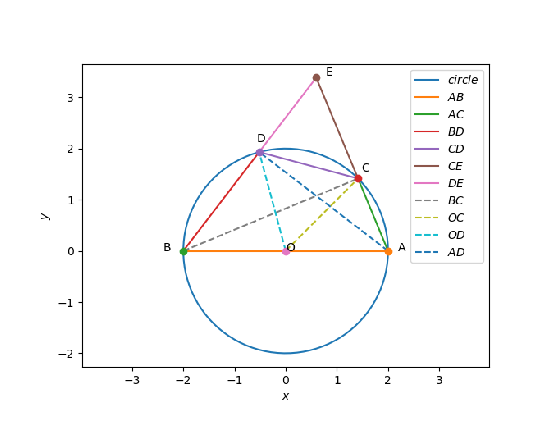
\includegraphics[width= \columnwidth]{Figure_1.eps}
\caption{Constructed using Python}
\label{fig:circle_python}
\end{figure}
%
and the equivalent latex-tikz code for Fig. \ref{fig:circle_latex} from
\begin{lstlisting}
figs/circle.tex
\end{lstlisting}
%
The above latex code can be compiled as a standalone document as
\begin{lstlisting}
figs/circle_fig.tex
\end{lstlisting}



\end{enumerate}